\documentclass[border=10pt]{standalone}
\usepackage{amssymb}
\usepackage[dvipsnames]{xcolor}
\usepackage{tikz}

\begin{document}
    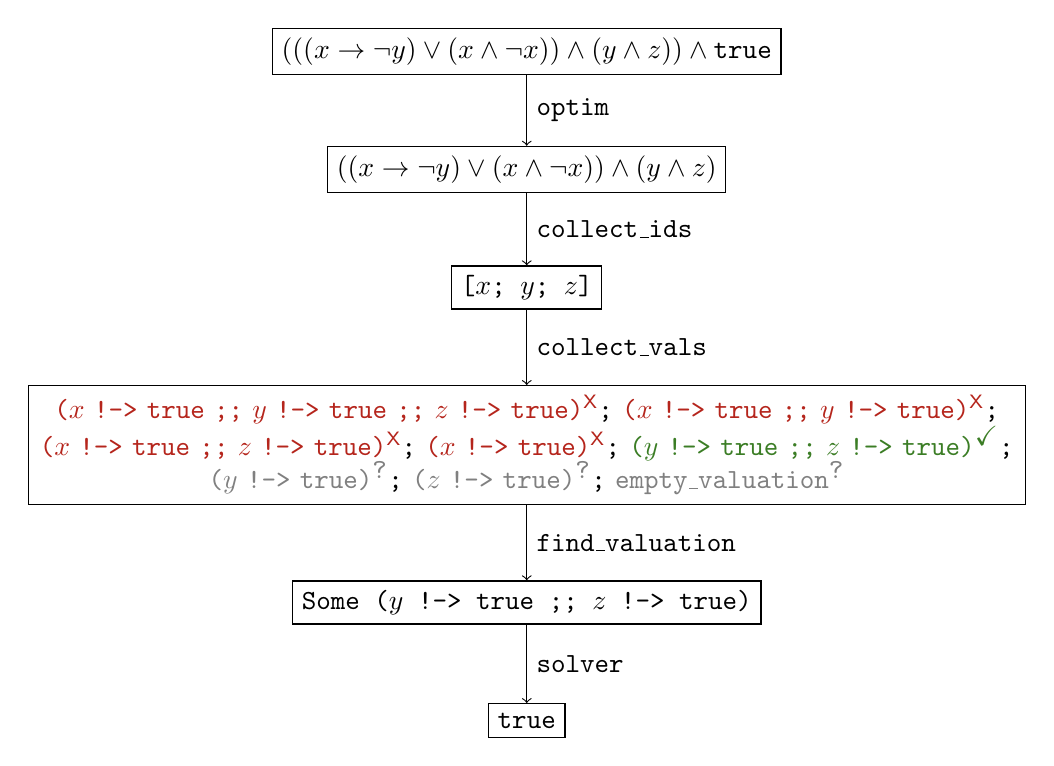
\begin{tikzpicture}
        \node[draw] (step1) at (0,0) {$(((x \rightarrow \neg y) \lor (x \land \neg x)) \land (y \land z)) \land \texttt{true}$};
        \node[draw] (step2) at (0,-1.5) {$((x \rightarrow \neg y) \lor (x \land \neg x)) \land (y \land z)$};
        \node[draw] (step3) at (0,-3) {\texttt{[$x$; $y$; $z$]}};
        \node[draw] (step4) at (0,-5) [text width=1.025\textwidth,align=center]{\texttt{\textcolor{BrickRed}{($x$ !-> true ;; $y$ !-> true ;; $z$ !-> true)$^\mathsf{X}$}; \textcolor{BrickRed}{($x$ !-> true ;; $y$ !-> true)$^\mathsf{X}$}; \textcolor{BrickRed}{($x$ !-> true ;; $z$ !-> true)$^\mathsf{X}$}; \textcolor{BrickRed}{($x$ !-> true)$^\mathsf{X}$}; \textcolor{OliveGreen}{($y$ !-> true ;; $z$ !-> true)$^{\checkmark}$};\\ \textcolor{gray}{($y$ !-> true)$^\textbf{?}$}; \textcolor{gray}{($z$ !-> true)$^\textbf{?}$}; \textcolor{gray}{empty\_valuation$^\textbf{?}$}}};
        \node[draw] (step5) at (0,-7) {\texttt{Some ($y$ !-> true ;; $z$ !-> true)}};
        \node[draw] (step6) at (0,-8.5) {\texttt{true}};

        \path[->] (step1) edge node[midway, right]{\texttt{optim}} (step2);
        \path[->] (step2) edge node[midway, right]{\texttt{collect\_ids}} (step3);
        \path[->] (step3) edge node[midway, right]{\texttt{collect\_vals}} (step4);
        \path[->] (step4) edge node[midway, right]{\texttt{find\_valuation}} (step5);
        \path[->] (step5) edge node[midway, right]{\texttt{solver}} (step6);
    \end{tikzpicture}
\end{document}
